\documentclass[10pt,svgnames,usenames,table]{beamer} %,handout si version papier
\NeedsTeXFormat{LaTeX2e} 

\usetheme[compress]{Singapore} % theme

\usepackage[french]{babel}
\usepackage[utf8x]{inputenc} % pour les accents (mettre latin1 pour
                            % windows au lieu de utf8)
\usepackage[T1]{fontenc}
\usepackage{amsmath,amsthm,amssymb}        % un packages mathématiques
\usepackage{xcolor}         % pour définir plus de couleurs
\usepackage{graphicx}       % pour insérer des figures
\usepackage{lmodern}
\usepackage{url}
	\urlstyle{sf}
\usepackage{lastpage}
\usepackage{endnotes}
\usepackage{listings}
\usepackage[french]{varioref}
\usepackage{wrapfig}
\usepackage{pdfpages}
\usepackage{verbatim}
\usepackage{graphicx}

%\usepackage[svgnames]{color}
%\definecolor{webdarkblue}{rgb}{0,0,0.4}
%\definecolor{webgreen}{rgb}{0,0.3,0}
%\definecolor{webblue}{rgb}{0,0,0.8}

\setbeamercolor{section in head/foot}{use=structure,bg=structure.fg!25!bg} % "Amélioration du jeu de couleur"
%\useoutertheme[subsection=true]{smoothbars} % Pour avoir un rappel de la subsection
\setbeamerfont{frametitle}{series=\bfseries}
\setbeamertemplate{frametitle}[default][center] % Titre centré et bien placé.


% "Fioriture de style" : qd <x-> dans les item, les autres en gris clair
\beamertemplatetransparentcovered


% Comportement des itemize
\setbeamertemplate{itemize item}[ball]
\setbeamertemplate{itemize subitem}[triangle]
\setbeamertemplate{itemize subsubitem}[circle]

%\renewcommand\sfdefault{cmss} % Polices

% Les block arrondis et ombrés dans la couleur que je veux
\setbeamertemplate{blocks}[rounded][shadow=true]
\definecolor{normalBlockColor}{RGB}{102,153,255}
\definecolor{normalTitleBlockColor}{RGB}{0,0,102}
\definecolor{normalBlockTextColor}{RGB}{255,255,255}
\definecolor{normalBlockTitleTextColor}{RGB}{255,255,255}
\definecolor{exampleBlockColor}{RGB}{202,251,197}
\definecolor{exampleTitleBlockColor}{RGB}{166,241,158}
\definecolor{exampleBlockTextColor}{RGB}{0,0,0}
\definecolor{exampleBlockTitleTextColor}{RGB}{0,120,0}
\definecolor{alertBlockColor}{RGB}{248,218,218}
\definecolor{alertTitleBlockColor}{RGB}{244,108,108}
\definecolor{alertBlockTextColor}{RGB}{0,0,0}
\definecolor{alertBlockTitleTextColor}{RGB}{120,0,0}
\setbeamercolor*{block title}{fg=normalBlockTitleTextColor,bg=normalTitleBlockColor}
\setbeamercolor*{block body}{fg=normalBlockTextColor,bg=normalBlockColor}
\setbeamercolor*{block title alerted}{fg=alertBlockTitleTextColor,bg=alertTitleBlockColor}
\setbeamercolor*{block body alerted}{fg=alertBlockTextColor,bg=alertBlockColor}
\setbeamercolor*{block title example}{fg=exampleBlockTitleTextColor,bg=exampleTitleBlockColor}
\setbeamercolor*{block body example}{fg=exampleBlockTextColor,bg=exampleBlockColor}
\setbeamerfont{block title}{size={}}



%------------ fin style beamer -------------------

% Faire apparaître un sommaire avant chaque section
% \AtBeginSection[]{
%   \begin{frame}
%   \frametitle{Plan}
%   \medskip
%   %%% affiche en début de chaque section, les noms de sections et
%   %%% noms de sous-sections de la section en cours.
%   \small \tableofcontents[currentsection, hideothersubsections]
%   \end{frame} 
% }


% Pour personnaliser la barre de navigation du dessous
\setbeamertemplate{navigation symbols}{
	%\insertslidenavigationsymbol
	%\insertframenavigationsymbol
	%\insertsubsectionnavigationsymbol
	\quad\textbf{\insertframenumber/\inserttotalframenumber} % Numéro de page
	%\insertsectionnavigationsymbol
	%\insertdocnavigationsymbol
	%\insertbackfindforwardnavigationsymbol
}
% Supprimer les icones de navigation (pour les transparents)
%\setbeamertemplate{navigation symbols}{}

% Mettre les icones de navigation en mode vertical (pour projection)
% \setbeamertemplate{navigation symbols}[vertical]

\newenvironment{itemize2}%
	{ \begin{list}%
		{$\bullet$}%
		{\setlength{\labelwidth}{30pt}%
		 \setlength{\leftmargin}{35pt}%
		 \setlength{\itemsep}{\parsep}}}%    
	{ \end{list} }

\def\siecle#1{\textsc{\romannumeral #1}\textsuperscript{e}~siècle} % => le \siecle{19}

\definecolor{codeBlue}{rgb}{0,0,1}
\definecolor{webred}{rgb}{0.5,0,0}
\definecolor{codeGreen}{rgb}{0,0.5,0}
\definecolor{codeGrey}{rgb}{0.6,0.6,0.6}
\definecolor{webdarkblue}{rgb}{0,0,0.4}
\definecolor{webgreen}{rgb}{0,0.3,0}
\definecolor{webblue}{rgb}{0,0,0.8}
\definecolor{orange}{rgb}{0.7,0.1,0.1}
\lstset{
      language=C,
      flexiblecolumns=true,
      numbers=left,
      stepnumber=1,
      numberstyle=\ttfamily\tiny,
      keywordstyle=\ttfamily\textcolor{blue},
      stringstyle=\ttfamily\textcolor{red},
      commentstyle=\ttfamily\textcolor{green},
      breaklines=true,
      extendedchars=true,
      basicstyle=\ttfamily\scriptsize,
      showstringspaces=false
    }

\usepackage{pdflscape} %% portrait
\usepackage[french]{varioref} % \vpageref
\usepackage{pgfplots}
\usepackage{framed}
\usepackage{mdframed}

\newcommand{\badet}{et}
\newcommand{\goodet}{\mathbin{\mathrm{et}}}

\lstdefinestyle{nonumbers}
{numbers=none}

\graphicspath{{img/}}
\definecolor{gris}{RGB}{228,228,228}
\definecolor{bleu}{RGB}{34,148,255}
\definecolor{darkgray}{rgb}{0.3,0.3,0.3}
\usefonttheme[onlymath]{serif} % to see the difference when I do mathsf

\logo{
\includegraphics[height=5mm]{logo_12-13-mini.png}}
\institute{Louvain-li-Nux}
\title{\textbf{Formation \LaTeX}\\
Introduction à l'écriture de document \textrm{\LaTeX}}
\author{Xavier \textsc{Lambein} \and Geoffroy \textsc{Jacquet}}

%\date{24 mars 2015}


% A changer (selon Arnaud) le utf8x pas aligné slide 12/30
% maketitle
%
%
\begin{document}

%%%%%%%%%%%% SIDA
\begin{landscape}
  \begin{frame}[noframenumbering,plain]
    \vspace{-.5cm}
    \hspace*{.1mm}
    
\includegraphics[page=1,height=\paperwidth]{latex_sida.pdf}
  \end{frame}
\end{landscape}
%%%%%%%%%%%%

\begin{frame}
  \begin{center}\Large
  Suivez cette présentation sur votre ordinateur :)
  
  \vspace{1cm}
  \fbox{\url{http://bit.ly/2cYF8sb}}
  \end{center}
\end{frame}


\begin{frame}
  \maketitle
  Merci à Jolan \textsc{Wolter} et Thomas \textsc{Vanzieleghem} pour avoir réalisé la première version de ces slides
  ainsi qu'à David \textsc{Ernst} et Matthieu \textsc{Baerts} pour avoir réalisé la deuxième version, ainsi qu'à Arnaud \textsc{Cerckel} et Benoît \textsc{Legat} pour avoir réalisé la troisième version.
\end{frame}

\AtBeginSection[]
  {
     \begin{frame}<beamer>
     \frametitle{\insertsection}
     \tableofcontents[hideothersubsections]
     \end{frame}
  }

\section{Introduction}
\subsection{Qu'est-ce que \LaTeX{}?}
\begin{frame}
\frametitle{Qu'est ce que \LaTeX}

\begin{itemize}
\item \TeX{} $ \Rightarrow$ programme de mise en page
\vspace{0.5cm}
\item \LaTeX{} $ \Rightarrow$ ensemble de commandes qui seront
 interprétées par le programme \TeX
 \vspace{0.5cm}
\item \LaTeX{} $ \neq$ WYSIWYG (What You See Is What You Get)
\end{itemize}

\end{frame}

\subsection{Pourquoi \LaTeX{}?}
\begin{frame}{Pourquoi \LaTeX{}?}

  \begin{itemize}
  	\item Qualité professionnelle de document
	\item Facilité d'emploi des :
	\begin{itemize}
		\item formules mathématiques
		\item table des matières
		\item références bibliographiques
		\item références croisées
		\item ...
	\end{itemize}
	\item Séparation entre contenu et forme
	\item Description du contenu indépendant de la forme
	\item Gratuit
	\item Stable, même pour les très gros documents
  \end{itemize}
\end{frame}

\begin{frame}{Pourquoi \LaTeX{}?}

\begin{figure}[htbp]
\begin{center}
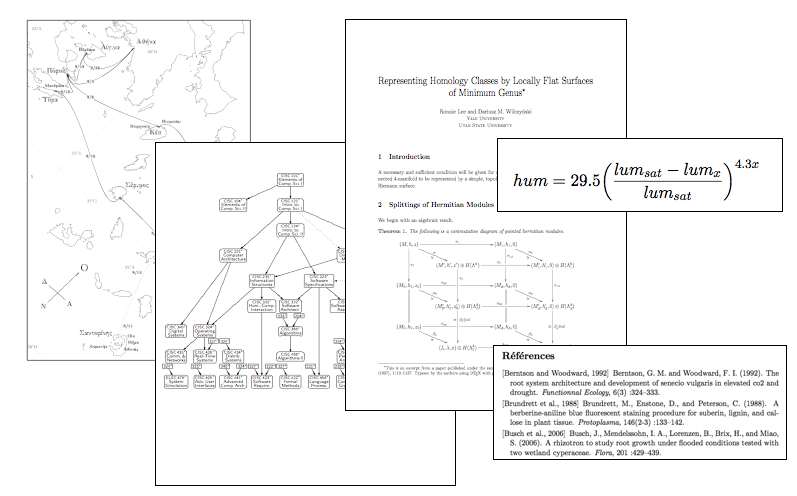
\includegraphics[height=6.5cm]{latex_exemples}
\end{center}
\end{figure}
\end{frame}

%-----------------------
\subsection{Pourquoi pas \LaTeX{}?}
\begin{frame}{Pourquoi pas \LaTeX{}?}

  \begin{itemize}
  	\item Les tableaux...
	\item Prise en main plus longue que pour traitement de texte WYSIWYG
	\item Je suis allergique à toute forme de code informatique
	\item J'ai des actions Microsoft
	\item Je ne trouve pas le ``\textbackslash'' sur mon clavier
  \end{itemize}
\end{frame}

\begin{frame}{Oui mais...}
  \begin{center}
    %\resizebox{\textwidth}{!}{
    \begin{tikzpicture}
      \begin{axis}[xmin=0, xmax=4, ymin=-2, ymax=5,
          xlabel={Expérience, maitrise}, ylabel=Productivité,
        legend style={at={(0.01,0.99)}, anchor=north west}]
        \addplot[smooth, color=blue]{x-0.05};
        \addlegendentry{\LaTeX}
        \addplot[smooth, color=red,domain=0:5]{sqrt(x)};
        \addlegendentry{Word}
        %\xlabel{Productivité}
        %\ylabel{Expérience/maitrise}
      \end{axis}
      \foreach \x/\com/\deltax/\deltay/\adj in {
        {1.1}/{Maintenant}/{0}/{0.8}/below,
        {2.2}/{Après la formation}/{0}/{0.4}/below,
        %{4.6}/{À l'heure de votre mémoire}/{0}/{1.2}/below
        {4.6}/{Au bout de queques semaines}/{0}/{1.2}/below
      } {
        %\fill \coord circle (100pt) node[\adj] {$\coord$};
        \draw[dashed] (\x,0) -- (\x+\deltax,\deltay) node[above] {\com};
        %\draw (\x+\deltax,\deltay) node {\com};
      }
    \end{tikzpicture}
    %}
  \end{center}
\end{frame}

%-----------------------
\subsection{Les Outils}
\begin{frame}{Quels logiciels pour utiliser \LaTeX{}?}

  \begin{itemize}
	  \item GNU/Linux
	  \begin{itemize}
	  	\item Distribution \LaTeX{} = \textbf{TeXLive}
		\item Éditeur de texte = \textbf{TeXMaker, LaTeXila, Kile}
	  \end{itemize}
	  \item Windows
	  \begin{itemize}
	  	\item Distribution \LaTeX{} = \textbf{TeXLive}
		\item Éditeur de texte = \textbf{TeXMaker}
	  \end{itemize}
	  \item Mac OS
	  \begin{itemize}
	  	\item Distribution \LaTeX{} = \textbf{MacTeX}
		\item Éditeur de texte = \textbf{TeXMaker, TeXShop, iTeXMac}
	  \end{itemize}
	  \item Dans votre navigateur
	  \begin{itemize}
		\item \textbf{\url{www.overleaf.com}}
  		\item \textbf{\url{www.sharelatex.com}}
	  \end{itemize}
  \end{itemize}
  Par simplicité, nous utiliserons \textbf{Overleaf} dans ce cours.
\end{frame}

\section{Les concepts de base}
\subsection{Les fichiers}

\begin{frame}{Les fichiers}

	\begin{center}
		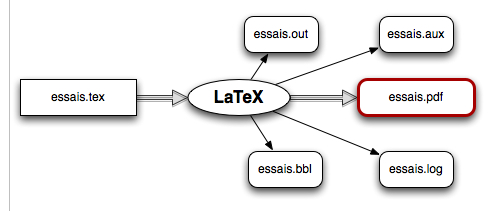
\includegraphics[height=3cm]{compilation.jpg}
	\end{center}

	\begin{itemize}
		\item Fichier source = essais\alert{\textbf{.tex}}
		\item Fichier de bibliographie = essais\alert{\textbf{.bib}}
		\item Lors de compilation $\rightarrow$ création de nombreux fichiers annexes
		\begin{itemize}
			\item style, class;
			\item structure du document;
			\item table des matières, liste des figures;
			\item liste des références;
			\item ...
		\end{itemize}
		\item Création d'un fichier essais\alert{\textbf{.pdf}}
	\end{itemize}
\end{frame}

%-----------------------
\subsection{La structure}

\begin{frame}[fragile,label=frame:structure]{Structure générale du document I}
\framesubtitle{Document minimal}
\small

\begin{lstlisting}[style=nonumbers]
\documentclass{article} %Type de document

%Préambule

\begin{document}
    %Corps du document
\end{document}
\end{lstlisting}
\begin{itemize}
	\item On charge les \textit{packages} et effectue certains réglages dans le préambule.
	\item On écrit le contenu de son docuement entre \lstinline|\begin{document}| et \lstinline|\end{document}|.
	\item Commentaires introduits par \%
\end{itemize}

\end{frame}

\begin{frame}[fragile]{Structure générale du document II}
\framesubtitle{Exemple de document type}
\small
\begin{tabular}{ll}
  Type de document &
  \lstinline|\documentclass[a4paper, 10pt]{article}|\\
  Utilisation de \textit{package} &
  \lstinline|\usepackage[utf8x]{inputenc}|\\
  Utilisation de \textit{package} &
  \lstinline|\usepackage[T1]{fontenc}|\\
  Utilisation de \textit{package} &
  \lstinline|\usepackage[french]{babel}|\\
  \textbf{Blanc pour la lisibilité} &\\
  Début du document &
  \lstinline|\begin{document}|\\
  Corps du document &
  \lstinline|Ceci est mon premier document en \LaTeX{}|\\
  Fin du document &
  \lstinline|\end{document}|\\
\end{tabular}
\end{frame}

\subsection{Commandes et environnements}
\begin{frame}[fragile]{Les commandes et environnements}
\begin{itemize}
\item \textbf{Commande} 
	\begin{itemize}
	\item Débute par \textbackslash
	\item S'applique à une partie du texte, délimité par des accolades
	\item Permet d'insérer des symboles
	\end{itemize}
	\begin{lstlisting}[style=nonumbers]
\commandName[options]{FirstParameter}...{LastParameter}
	\end{lstlisting}
	\begin{center}
	\begin{tabular}{llll}
	\lstinline|\LaTeX{}| & \LaTeX{} & \lstinline|\textbf{texte}| & \textbf{texte}
	\end{tabular}
	\end{center}
\item \textbf{Environnement}
	\begin{itemize}
	\item S'applique à des portions de texte et applique une règle de mise en page,\dots
	\item Délimité par \lstinline|\begin| et \lstinline|\end|
	\end{itemize}
	\begin{lstlisting}[style=nonumbers]
\begin{EnvironnementName}[options]

\end{EnvironnementName}
	\end{lstlisting}
\end{itemize}
\end{frame}
%-----------------------

\subsection{Les classes}

\begin{frame}[fragile]{Les principales classes de document}
\begin{tabular}{lp{8cm}}
  \textbf{article} & pour les articles de journaux scientifiques, présentations, rapports courts,\dots \\
  \textbf{report} & pour de plus long rapports de plusieurs chapitres, petits livres, thèses,\dots \\
  \textbf{book} & pour de vrais livres.\\
  \textbf{letter} & pour écrire des lettres.\\
  \textbf{beamer} & pour écrire des présentations (comme celle-ci).
\end{tabular}
\vspace{1cm}
\begin{center}
\verb|\documentclass[a4paper,10pt]{|\alert{\texttt{article}}\verb|}|\\
\end{center}
\end{frame}

\subsection{Les options}

\begin{frame}[fragile]{Les principales options de document}
\begin{tabular}{lp{8cm}}
  \textbf{10pt, 11pt, 12pt} & pour la taille de police.\\
  \textbf{a4paper, a5paper} & pour la taille de page.\\
  \textbf{onecolumn, twocolumn} & pour faire plusieurs colonnes.\\
  \textbf{landscape} & pour une mise en page paysage.\\
  \textbf{twoside} & pour des marges de livre
\end{tabular}
\vspace{1cm}
\begin{center}
\verb|\documentclass[|\alert{\texttt{a4paper,10pt}}\verb|]{article}|\\
\end{center}
\end{frame}

\subsection{Les packages}

\begin{frame}[fragile]{Les packages}
\begin{itemize}
\item Les \textbf{packages} sont des extensions contenant de nouveaux environnements et commandes
\item Appel du package dans le \textit{préambule} à l'aide de la commande \lstinline|\usepackage[options]{packageName}|
\end{itemize}
\vskip2em
\begin{tabular}{ll}
\lstinline|\usepackage[utf8]{inputenc}| & Utilisation des caractères accentués \\
\lstinline|\usepackage[T1]{fontenc}| & Permet d'utiliser tous les caractères du clavier \\
\lstinline|\usepackage[french]{babbel}| & Spécifie la langue (français ici)
\end{tabular}

\end{frame}

\subsection{La structure}
\begin{frame}[fragile]{La structure logique du document}
	\begin{itemize}
		\item Structure logique du document uniquement
		\item \LaTeX{} se charge de la numérotation et de la mise en page\\
	\end{itemize}
	\vspace{1cm}

	\lstinline|\part{}|\\
	\hspace{1cm} \lstinline|\chapter{}| \hspace{2cm}$\Longrightarrow$ \textcolor{red}{uniquement \textit{book} et \textit{report}}\\
	\hspace{2cm} \lstinline|\section{}|\\
	\hspace{3cm} \lstinline|\subsection{}| \\
	\hspace{4cm} \lstinline|\subsubsection{}| \\
	\hspace{5cm} \lstinline|\paragraph{}	| \\

\end{frame}

\begin{frame}[fragile]{La structure logique du document}
\framesubtitle{Exemple}
	\begin{columns}
      \begin{column}{0.5\textwidth}
        \begin{lstlisting}[style=nonumbers]
\part{Ma partie}
\section{Une section de mon document}
\subsection{Ma sous-section}
        \end{lstlisting}
      \end{column}
      \begin{column}{0.5\textwidth}
        \fbox{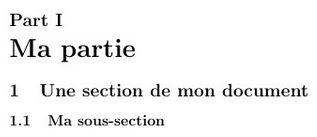
\includegraphics[width=1\textwidth]{structure_logique.png}}
      \end{column}
	\end{columns}
\end{frame}

%-----------------------
\section{Mise en page générale} %TODO: faire ca plus clairement

\subsection{Titre}
\begin{frame}[fragile]{Titre}
	\begin{itemize}
		\item Informations données dans \lstinline|\author{}|, \lstinline|\date{}| and \lstinline|\title{}| \textbf{avant} le \lstinline|\begin{document}|
		\item Création de la page de titre avec \lstinline|\maketitle| \textbf{après} le \lstinline|\begin{document}|
	\end{itemize}
	\begin{columns}
      \begin{column}{0.5\textwidth}
        \begin{lstlisting}[style=nonumbers]
\title{Formation \LaTeX}

% Séparer les auteurs avec \and
\author{Xavier \textsc{Lambein}
        \and Geoffroy \textsc{Jacquet}}

                    % today
\date{24 mars 2015} % fixed data
\date{}             % no date
        \end{lstlisting}

        \begin{lstlisting}[style=nonumbers]
\begin{document}

\maketitle
        \end{lstlisting}
      \end{column}
      \begin{column}{0.5\textwidth}
        
\includegraphics[scale=0.35]{pdg.png}
      \end{column}
	\end{columns}
\end{frame}

\subsection{Le résumé ou abstract}
\begin{frame}[fragile]{Le résumé ou abstract}
	\begin{itemize}
		\item L'environnement \lstinline|abstract| permet de mettre en page un résumé au début du document.
	\end{itemize}
	\begin{columns}
      \begin{column}{0.5\textwidth}
        \begin{lstlisting}[style=nonumbers]
\begin{document}
...
\begin{abstract}
  Voici un résumé succint du contenu
  de mon document.
\end{abstract}
...
\end{document}
        \end{lstlisting}
      \end{column}
      \begin{column}{0.5\textwidth}
				\begin{abstract}
					Voici un résumé succint du contenu de mon document.
				\end{abstract}
      \end{column}
	\end{columns}
\end{frame}

\subsection{La table des matières}
\begin{frame}[fragile]{Table des matières}
	\begin{itemize}
		\item La commande \lstinline|\tableofcontents| suffit pour générer toute la table des matières
	\end{itemize}
	\begin{columns}
      \begin{column}{0.6\textwidth}
        \begin{lstlisting}[style=nonumbers]
\begin{document}

\tableofcontents % Table des matières

\section{Introduction}
Ceci est mon premier document en \TeX{}

\section{Le vif du sujet}
Le sujet est en or mais pas le vif.

\subsection{Mais quel est le sujet ?}
\LaTeX{}, ce logiciel d'exception !

\end{document}
        \end{lstlisting}
      \end{column}
      \begin{column}{0.4\textwidth}
        \begin{center}
          \fbox{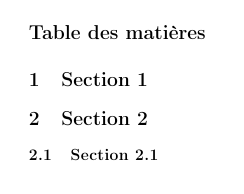
\includegraphics[width=0.9\textwidth]{table.png}}
        \end{center}
      \end{column}
	\end{columns}
\end{frame}

\subsection{Exercice 1}
\begin{frame}[fragile]{Premier exercice}
  
	\begin{columns}[T]
    \begin{column}{0.5\textwidth}
      \begin{center}\large
        Exercice sur Overleaf\footnotemark{}:
        
        \vspace{0.25cm}
        \fbox{\url{http://bit.ly/2ecAO9b}}
      \end{center}
    \end{column}
    \begin{column}{0.5\textwidth}
      \begin{center}\large
        \vfill
        Exemple de résultat:
        
        \vspace{0.25cm}
        \fbox{\url{http://bit.ly/2dL13kb}}
      \end{center}
        \vfill
    \end{column}
	\end{columns}
  \footnotetext{Cliquez sur \og{}Clone this project\fg{} pour commencer à écrire.}
  \vspace{0.25cm}
  
  Dans cet exercice, on vous invite à:
  \begin{itemize}
	  \item créer un \textbf{titre} de document;
	  \item changer la \textbf{taille de police} du document;
	  \item ajouter un \textbf{résumé} (abstract);
	  \item définir la structure de votre document avec quelques \textbf{sections} et \textbf{sous-sections};
	  \item écrire un peu de \textbf{texte};
	  \item générer la \textbf{table des matières} au début de votre document.
  \end{itemize}
\end{frame}


%-----------------------
\subsection{Paragraphes}
\begin{frame}[fragile]{Les paragraphes avec \LaTeX{}}
	\begin{itemize}
	\item Pour créer un nouveau paragraphe, il suffit de faire deux retours à la ligne
    \begin{columns}
      \begin{column}{0.4\textwidth}
    	  \begin{lstlisting}[style=nonumbers]
Premier paragraphe.
Ceci est toujours le premier
paragraphe.

Second paragraphe.
	      \end{lstlisting}
      \end{column}
      \begin{column}{0.6\textwidth}
        \setlength{\parindent}{1.5em}
        \par{}Premier paragraphe.
        Ceci est toujours le premier paragraphe.

        Second paragraphe.
        \setlength{\parindent}{0pt}
      \end{column}
    \end{columns}
  \end{itemize}
\end{frame}

\subsection{Paragraphes}
\begin{frame}[fragile]{Les paragraphes avec \LaTeX{}}
\framesubtitle{Les styles de paragraphes}
	\begin{itemize}
	\setlength\itemsep{1em}
	\item Par défaut, le style des paragraphes est défini par la langue

	\item Ajouter de l'espace entre les paragraphes. Attention: ce package retire l'indentation.
	  \begin{columns}
	    \begin{column}{0.4\textwidth}
    	  \begin{lstlisting}[style=nonumbers]
\usepackage{parskip}
	      \end{lstlisting}
	    \end{column}
	    \begin{column}{0.6\textwidth}
        \par{}Ces deux paragraphes ont maintenant un espace entre eux.
        \vspace{0.5em}

        \par{}Cependant, l'indentation a disparue.
	    \end{column}
    \end{columns}
  
	\item Changer (ou remettre) l'indentation des paragraphes
	  \begin{columns}
	    \begin{column}{0.4\textwidth}
	      \begin{lstlisting}[style=nonumbers]
\setlength{\parindent}{30pt}
    	  \end{lstlisting}
	    \end{column}
	    \begin{column}{0.6\textwidth}
        \setlength{\parindent}{30pt}
        \par{}Ce paragraphe est fortement indenté.
        \setlength{\parindent}{0em}
	    \end{column}
    \end{columns}
    
  \item Ajouter un espace interligne
	  \begin{columns}
	    \begin{column}{0.4\textwidth}
        \begin{lstlisting}[style=nonumbers]
\usepackage{setspace}
\setstretch{1.5}
        \end{lstlisting}
	    \end{column}
	    \begin{column}{0.6\textwidth}
        \setlength{\parindent}{1.5em}
        \setstretch{1.5}
        \par{}Ce paragraphe a un espace interligne plus important que les autres.
        \setlength{\parindent}{0em}
	    \end{column}
    \end{columns}
  \end{itemize}
  \setstretch{1.0}
\end{frame}

\begin{frame}[fragile]{Les paragraphes avec \LaTeX{}}
  \framesubtitle{Alignement d'un paragraphe}
  \begin{itemize}
  	\item Les environnements \lstinline|center|, \lstinline|flushright| et \lstinline|flushleft| permettent d'aligner un paragraphe.
    \begin{columns}
      \begin{column}{0.4\textwidth}
        \begin{lstlisting}[style=nonumbers]
Justifié; c'est le comportement par défaut de \LaTeX{}  

\begin{center}
  Centré
\end{center}

\begin{flushright}
  Aligné à droite
\end{flushright}

\begin{flushleft}
  Aligné à gauche, mais pas justifié, comme vous pouvez le voir
\end{flushleft}
        \end{lstlisting}
      \end{column}
      \begin{column}{0.6\textwidth}
        \begin{mdframed}
          Justifié; c'est le comportement par défaut de \LaTeX{} 

          \begin{center}
            Centré
          \end{center}

          \begin{flushright}
            Aligné à droite
          \end{flushright}

          \begin{flushleft}
            Aligné à gauche, mais pas justifié, comme vous pouvez le voir
          \end{flushleft}
        \end{mdframed}
      \end{column}
    \end{columns}
  \end{itemize}	
\end{frame}


%-----------------------
\subsection{Les polices}

\begin{frame}[fragile]{Jouer avec les fontes}
\framesubtitle{Changer la taille de police}
\begin{itemize}
	\item \lstinline|{\small text}| pour changer la taille du texte à l'intérieur
	\item \lstinline|\small| pour changer tout le texte jusqu'au prochain appel de \lstinline|\normalsize| 
\end{itemize}
\begin{tabular}{ll}
\lstinline|{\tiny polygenelubricants}| & {\tiny polygenelubricants} \\
\lstinline|{\small polygenelubricants}| & {\small polygenelubricants} \\
\lstinline|{\normalsize polygenelubricants}| & {\normalsize polygenelubricants} \\
\lstinline|{\large polygenelubricants}| & {\large polygenelubricants} \\
\lstinline|{\Large polygenelubricants}| & {\Large polygenelubricants} \\
\lstinline|{\LARGE polygenelubricants}| & {\LARGE polygenelubricants} \\
\lstinline|{\huge polygenelubricants}| & {\huge polygenelubricants} \\
\lstinline|{\Huge polygenelubricants}| & {\Huge polygenelubricants} \\
\end{tabular}
\end{frame}

\begin{frame}[fragile]{Jouer avec les fontes}
\framesubtitle{Changer le type et style de police}

\begin{itemize}
\item Type de police
\begin{center}
\begin{tabular}{ll}
\lstinline|\textrm{Serif (par défaut)}| & \textrm{Serif (par défaut)} \\
\lstinline|\textsf{Sans serif}| & \textsf{Sans serif} \\
\lstinline|\texttt{Machine à écrire}| & \texttt{Machine à écrire}
\end{tabular}
\end{center}

\item Style de police
\begin{center}
\begin{tabular}{ll}
\lstinline|\emph{Emphase}| & \emph{Emphase} \\
\lstinline|\textbf{Gras}| & \textbf{Gras} \\
\lstinline|\textsl{Italique}| & \textsl{Italique} \\
\lstinline|\textsc{Petites majuscules}| & \textsc{Petites majuscules}
\end{tabular}
\end{center}
\end{itemize}
\end{frame}


%-----------------------
\subsection{Listes}
\begin{frame}[fragile]
  \frametitle{Itemize et enumerate}
  \begin{itemize}
    \item Pour faire des listes à puce, utiliser l'environnement \lstinline|itemize|.
    \begin{columns}
      \begin{column}{0.45\textwidth}
        \begin{lstlisting}[style=nonumbers]
\begin{itemize}
  \item Un chat;
  \item une poule;
  \item un chien.
\end{itemize}
        \end{lstlisting}
      \end{column}
      \begin{column}{0.45\textwidth}
        \begin{itemize}
          \item Un chat;
          \item une poule;
          \item un chien.
        \end{itemize}
      \end{column}
    \end{columns}

    \item Pour faire des listes numerotées, utiliser l'environnement \lstinline|enumerate|.
    \begin{columns}
      \begin{column}{0.45\textwidth}
        \begin{lstlisting}[style=nonumbers]
\begin{enumerate}
  \item Mettez de l'eau.
  \item Chauffer l'eau.
  \item Mettez les pasta.
\end{enumerate}
        \end{lstlisting}
      \end{column}
      \begin{column}{0.45\textwidth}
        \begin{enumerate}
          \item Mettez de l'eau.
          \item Chauffer l'eau.
          \item Mettez les pâtes.
        \end{enumerate}
      \end{column}
    \end{columns}
  \end{itemize}
\end{frame}

\begin{frame}[fragile]
  \frametitle{Description}
  \begin{itemize}
    \item L'environnement \lstinline|description| permet de faire des définitions.
    \begin{lstlisting}[style=nonumbers]
\begin{description}
  \item[ODT] Open Document Text.
  \item[ODS] Open Document Spreadsheet.
  \item[ODP] Open Document Presentation.
\end{description}
    \end{lstlisting}
    \begin{description}
      \item[ODT] Open Document Text.
      \item[ODS] Open Document Spreadsheet.
      \item[ODP] Open Document Presentation.
    \end{description}
\end{itemize}
\end{frame}

\subsection{Divers}
\begin{frame}[fragile]{Divers I}
  \frametitle{Divers}
  \begin{itemize}
  \item Caractères spéciaux utilisés par \LaTeX
  
  \begin{tabular}{cccccccccc}
  \$ & \& & \% & \# & \_ & \{ & \} & \~{} & \^{} & \textbackslash \\
  \lstinline|\$| & \lstinline|\&| & \lstinline|\%| & \lstinline|\#| & \lstinline|\_| & \lstinline|\{| & \lstinline|\}| & \lstinline|\~{}| & \lstinline|\^{}| & \lstinline|\textbackslash|
  \end{tabular}
  

 \item Tirets
   \begin{tabular}{llp{0.5\textwidth}}
     \lstinline|-| & court & Jean-Patrick\\
     \lstinline|--| & moyen ou semi-cadratin & 1984--2015\\
     \lstinline|---| & cadratin & le \LaTeX{} --- c'est chouette --- a été créé par Leslie Lamport\\
   \end{tabular}
 \end{itemize}
\end{frame}

\begin{frame}[fragile]{Divers II}
\begin{itemize}
	\item Accents 
	\\
	\begin{tabular}{ccccccc}
		\lstinline|\'e| & \lstinline|\`e| & \lstinline|\^e| & \lstinline|\~n| & \lstinline|\=a| & \lstinline|\.e| & \lstinline|\c c| \\ 
		\'e & \`e & \^e & \~n & \=a & \.e & \c c \\
		\lstinline|\u e| & \lstinline|\v e| & \lstinline|\H a| & \lstinline|\d a| & \lstinline|\b a| & \lstinline|\t a| &\\
		\u e & \v e & \H a & \d a & \b a & \t a &
	\end{tabular}
	\item Autres caractères
	\begin{itemize}
		\item \lstinline|M\up{me}| pour M\up{me}
		\item \lstinline|1\ier{} 2\ieme{}| pour 1\ier{} et 2\ieme{}
		\item \lstinline|\no \No| pour \no et \No
		\item \lstinline|\degres C| pour \degres C
		\item \lstinline|\og{} \fg{}| pour \og{} \fg{}. \textcolor{red}{Attention, ne pas utiliser "}
	\end{itemize}
\end{itemize}
\end{frame}

%-----------------------
\subsection{Exercice 2}
\begin{frame}[fragile]{Deuxième exercice}
  \begin{columns}[T]
    \begin{column}{0.5\textwidth}
      \begin{center}\large
        Exercice sur Overleaf\footnotemark{}:
        
        \vspace{0.25cm}
        \fbox{\url{http://bit.ly/2dJSO9A}}
      \end{center}
    \end{column}
    \begin{column}{0.5\textwidth}
      \begin{center}\large
        \vfill
        Exemple de résultat:
        
        \vspace{0.25cm}
        \fbox{\url{http://bit.ly/2e1LpR2}}
      \end{center}
        \vfill
    \end{column}
  \end{columns}
  \footnotetext{Cliquez sur \og{}Clone this project\fg{} pour commencer à écrire.}
  \vspace{0.25cm}
  
  Dans cet exercice, on vous invite à:
  \begin{itemize}
    \item faire quelques paragraphes avec interligne double;
    \item faire un paragraphe centré;
    \item mettre un des mot en très grand, et un autre en très petit;
    \item faire une liste numérotée avec un type de police différent pour chaque élément;
    \item faire une list à puce avec un style de police différent pour chaque élément;
    \item combiner ce qui a été vu jusqu'ici à votre guise.
  \end{itemize}
\end{frame}

%-----------------------
\section{Les environnements flottants}
\subsection{Les figures}

\begin{frame}[fragile,allowframebreaks]
  \frametitle{Figures}
  \begin{itemize}
  
  \item Utilisation du package \lstinline|\usepackage{graphicx}|
  \item Insertion de l'image avec \lstinline|\includegraphics[options]{filename.ext}|  
  
  \item \textbf{Non-flottant}
  
    Référencement par ``ci-dessous'', \dots
    \begin{lstlisting}[style=nonumbers]
\begin{center}
  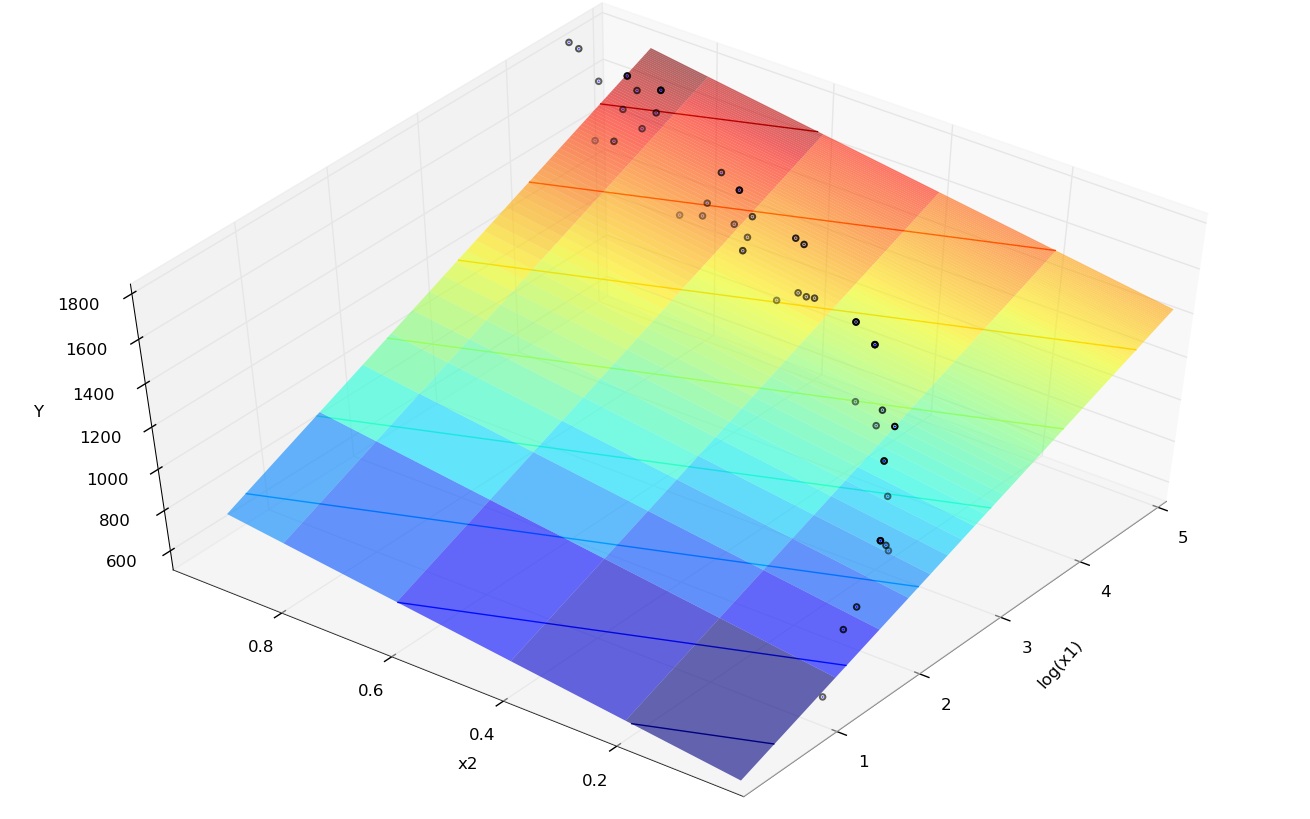
\includegraphics{image.jpg}
\end{center}
    \end{lstlisting}
  
  \item \textbf{Flottant}
  	\begin{itemize}
  		\item Environnement \lstinline|figure|
  		\item Ajout d'une référence par \lstinline|\label{...}|
    	\item Référencement par \lstinline|voir figure~\ref{fig:graphique}|
    	\item Ajout d'une légende par \lstinline|\caption{...}|
    \end{itemize}
    \begin{lstlisting}[style=nonumbers]
\begin{figure}[!ht]
  \centering
  \includegraphics{graph.png}
  \caption{Voici un beau graphique}
  \label{fig:graphique}
\end{figure}
    \end{lstlisting}
    
 
  \item \textbf{Scaling}
    \begin{lstlisting}[style=nonumbers]
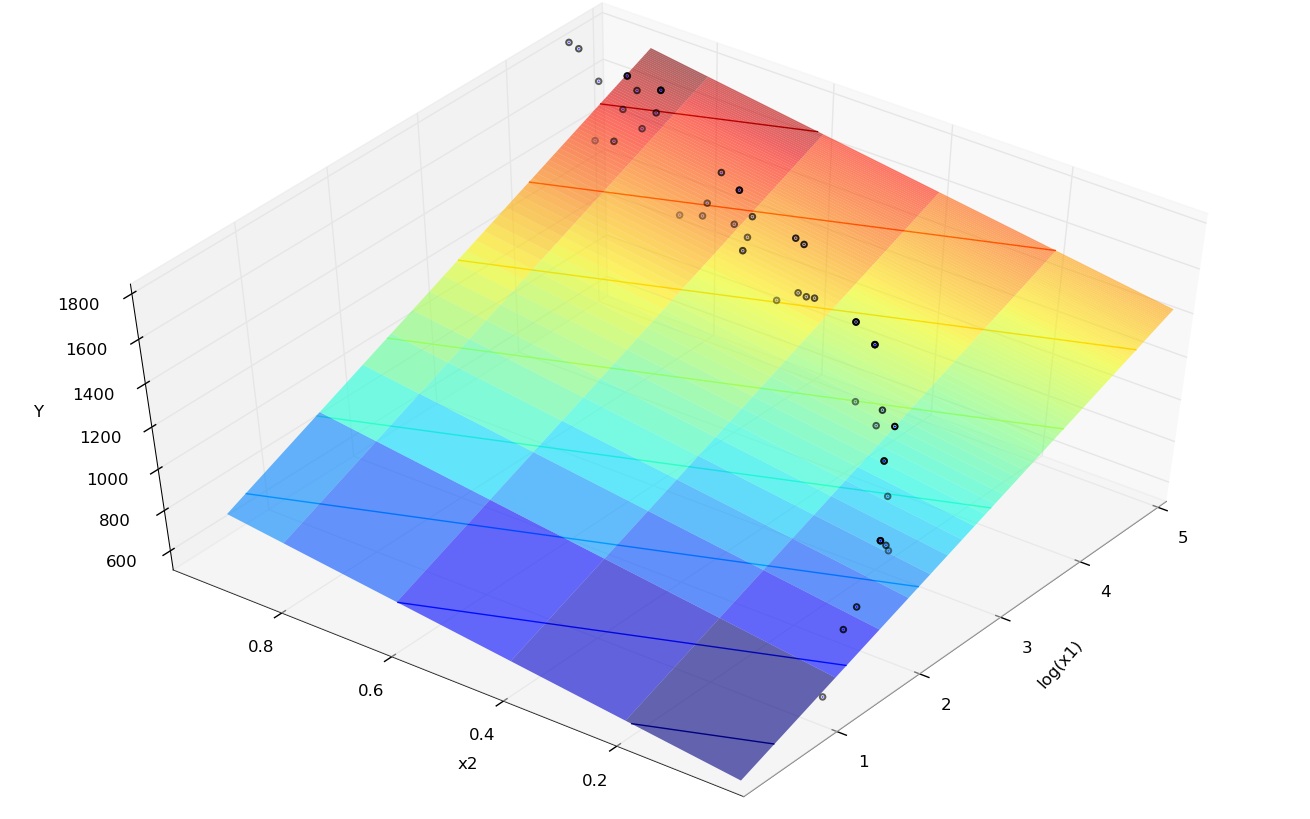
\includegraphics[width=\textwidth]{image.jpg} % Largeur d'une ligne de texte
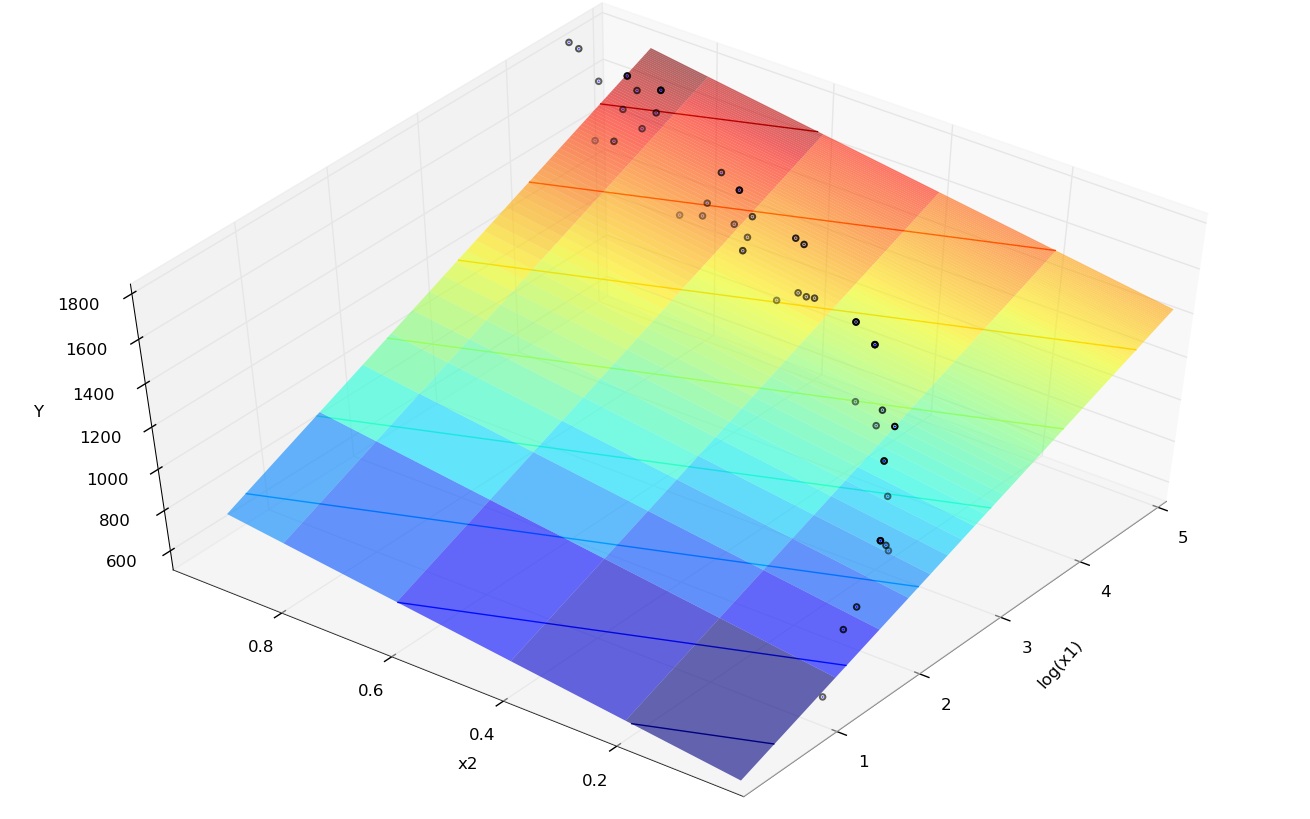
\includegraphics[height=4cm]{image.jpg} % Hauteur de 4cm
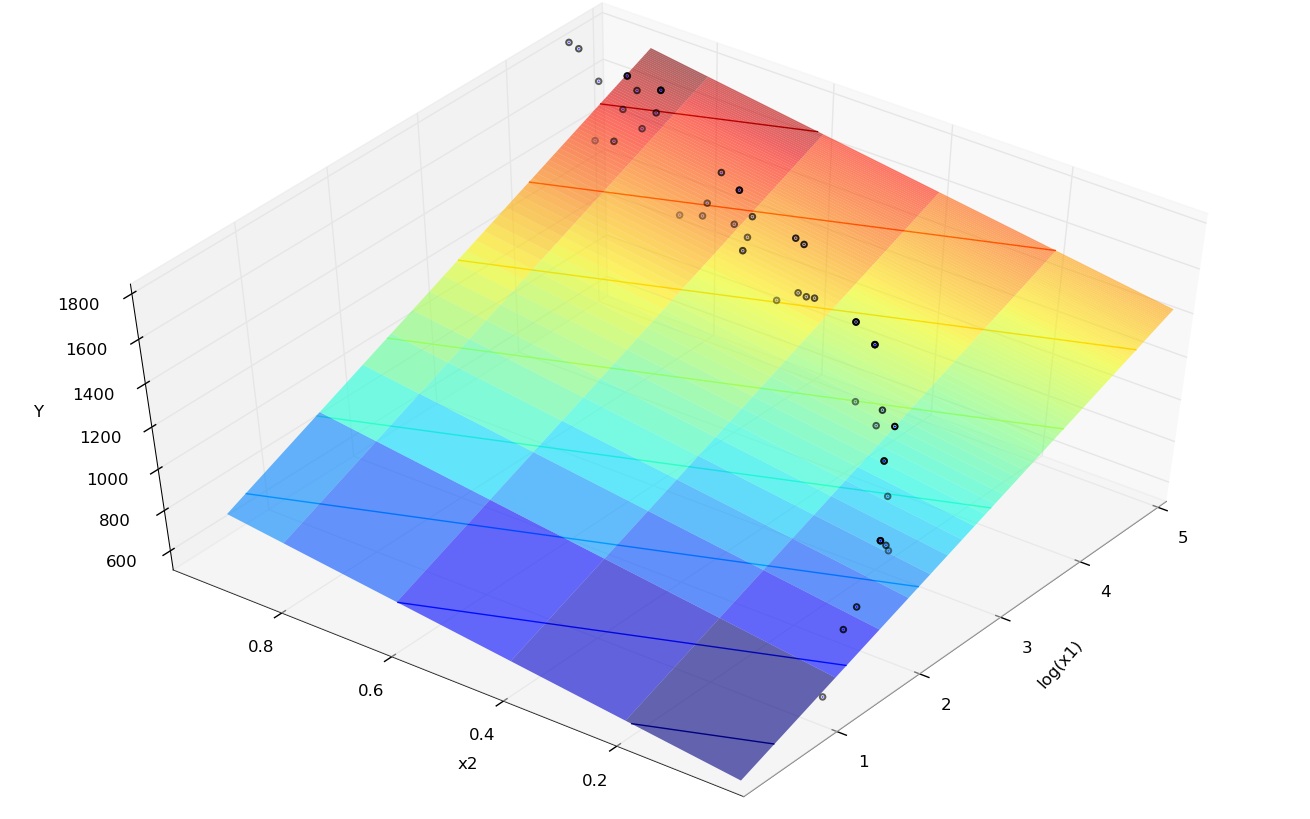
\includegraphics[scale=0.5]{image.png} % taille / 2
    \end{lstlisting}

  \vspace{2em}


\end{itemize} 
\begin{quote}
  1992: Extensive testing shows that 98.3\% of the time
  no matter which of the
  \lstinline|[h]|,
  \lstinline|[t]|,
  \lstinline|[b]|, or
  \lstinline|[p]|
  options is used,
  \LaTeX{} will put your \lstinline|table| at the end of the document.

  \vspace{1em}
  \hfill
  \em
  \begin{minipage}{8cm}
    DAVID F. GRIFFITHS and DESMOND J. HIGHAM, Great Moments in \LaTeX{} History (1997)
  \end{minipage}
\end{quote}

\end{frame}


\begin{frame}[fragile]{Exemple de figure}

\begin{columns}
    \begin{column}{0.5\textwidth}
Sur la figure~\ref{fig:ucl}, vous pouvez voir le logo UCL
mis a \SI{50}{\percent} de la largeur du texte.

\begin{figure}[!ht]
    \centering
        
\includegraphics[width=0.50\textwidth]{logo-ucl.eps}
    \caption{Voici le logo UCL}
    \label{fig:ucl}
\end{figure}
\end{column}

\begin{column}{0.5\textwidth}
\begin{lstlisting}[style=nonumbers]

Sur la figure~\ref{fig:ucl}, vous pouvez 
voir le logo UCL mis a \SI{50}{\percent}
de la largeur du texte.

\begin{figure}[!ht]
    \centering
        
\includegraphics[width=0.50\textwidth]{logo-ucl.eps}
    \caption{Voici le logo UCL}
    \label{fig:ucl}
\end{figure}
\end{lstlisting}
\end{column}
\end{columns}

\end{frame}


\subsection{Les tableaux} 
\begin{frame}[fragile,allowframebreaks]
  \frametitle{Tableaux}
  \begin{itemize}
  \item Utilisation de l'environnement \lstinline|tabular|
  \item \textbf{Non-flottant}
  
    Référencement par ``ci-dessous'', \dots
    \begin{lstlisting}[style=nonumbers]
  \begin{tabular}{...}
    ...
  \end{tabular}
    \end{lstlisting}
    
  \item \textbf{Flottant}
  	\begin{itemize}
  		\item Environnement \lstinline|table|
    	\item Référencement par \lstinline|voir tableau~\ref{tab:data}|
    \end{itemize}
    \begin{lstlisting}
\begin{table}
  \centering
  \begin{tabular}{...}
    ...
  \end{tabular}
  \caption{Voici un beau tableau}
  \label{tab:data}
\end{table}
    \end{lstlisting}
    
  \item \textbf{Code}
  	\begin{lstlisting}[style=nonumbers]
\begin{tabular}{<colonnes>}
  	<lignes>
\end{tabular}
  	\end{lstlisting}
  	\begin{itemize}
  		\item Définition de l'alignement des <colonnes> par :
  			\begin{itemize}
  				\item un \lstinline|l| pour aligner à gauche (\textit{left})
  				\item un \lstinline|c| pour centrer (\textit{center})
  				\item un \lstinline|r| pour aligner à droite (\textit{right})
  				\item un \lstinline|p{<largeur>}| pour un texte justifié sur une largeur donnée
  			\end{itemize}
  		\item Une ligne verticale est tracée par \lstinline|||
  		\item Le contenu des <lignes> est séparé par colonnes par \lstinline|&|
  		\item Une <ligne> se termine par \lstinline|\\|
  		\item Une ligne horizontalle est tracée par \lstinline|\hline|
  	\end{itemize}
    \begin{lstlisting}
\begin{tabular}{|lcr|}
  \hline
  A & B & C\\
  \hline
  a & b & c\\
  $\alpha$ & $\beta$ & $\gamma$\\
  \hline
\end{tabular}
    \end{lstlisting}
  \item \textbf{Rendu}
  
\begin{tabular}{|lcr|}
  \hline
  A & B & C\\
  \hline
  a & b & c\\
  $\alpha$ & $\beta$ & $\gamma$\\
  \hline
\end{tabular}
  \end{itemize}
\end{frame}



\begin{frame}[fragile]{Exemple de tableau}
\begin{footnotesize}
\begin{lstlisting}[style=nonumbers]
\begin{table}[!ht]
    \begin{center}
            \begin {tabular}{|l||c|} %% 2 columns
            \hline
                \textit{Inventaire} & \textbf{Nombre} \\
            \hline
                Chemises  & 4   \\
                Pulls     & 12  \\
                Pantalons & 1   \\
            \hline
            \end{tabular}
        \caption{Tableau relatif a l'inventaire}
    \end{center}
\end{table}
\end{lstlisting}
\end{footnotesize}
\begin{center}
\fbox{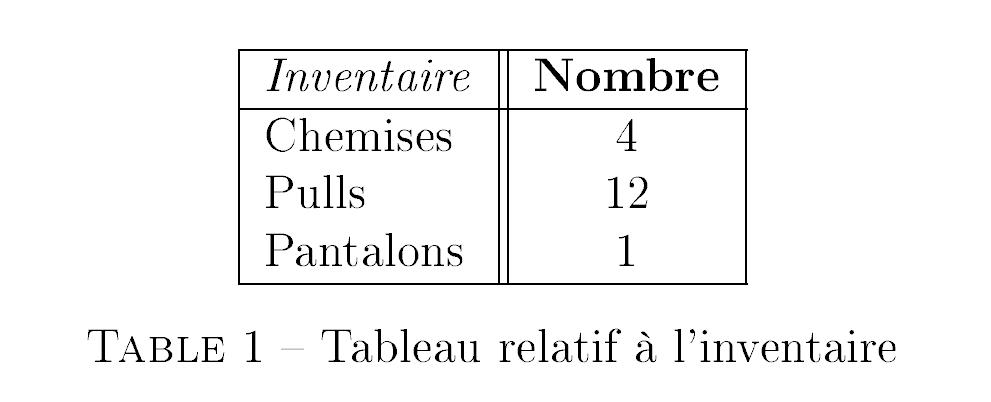
\includegraphics[width=0.6\textwidth]{table.jpg}}
\end{center}
\end{frame}

\subsection{Exercice 3}
\begin{frame}[fragile]{Troisième exercice}
  
	\begin{columns}[T]
    \begin{column}{0.5\textwidth}
      \begin{center}\large
        Exercice sur Overleaf\footnotemark{}:
        
        \vspace{0.25cm}
        \fbox{\url{http://bit.ly/2daowce}}
      \end{center}
    \end{column}
    \begin{column}{0.5\textwidth}
      \begin{center}\large
        \vfill
        Exemple de résultat:
        
        \vspace{0.25cm}
        \fbox{\url{http://bit.ly/2egnhhy}}
      \end{center}
        \vfill
    \end{column}
	\end{columns}
  \footnotetext{Cliquez sur \og{}Clone this project\fg{} pour commencer à écrire.}
  \vspace{0.25cm}
  
  Dans cet exercice, on vous invite à:
  \begin{itemize}
	  \item créer une \textbf{section} de document : 
	  \begin{itemize}
	  	\item écrire un peu de \textbf{texte};
	  	\item ajouter une \textbf{figure} (flottant) avec une \textbf{légende} (caption) et \textbf{référence} (label);
	  	\item écrire un peu de \textbf{texte} et faire \textbf{référence} à votre image;
	  \end{itemize} 
	  \item créer une \textbf{section} de document : 
	  \begin{itemize}
	  	\item écrire un peu de \textbf{texte} et faire \textbf{référence} à votre \textbf{tableau} (qui sera écrit plus bas);
	  	\item ajouter un \textbf{tableau} (flottant) avec une \textbf{légende} (caption) et \textbf{référence} (label);
	  \end{itemize}
  \end{itemize}
\end{frame}



%%%%%%%%%%%%%%%%%%%%%%%%%%%
\section{Références}

\subsection{Références des éléments du texte}
\begin{frame}[fragile]
\frametitle{\insertsubsection}
\begin{itemize}
  \item Facile de faire référence à un numéro et la page d'une section et d'un environnement (\texttt{figure}, \texttt{equation}, \texttt{table}).
  \item D'un coté une étiquette :
    \begin{itemize}
      \item \lstinline|\label{id}|.
    \end{itemize}
  \item De l'autre une référence à cette étiquette :
    \begin{itemize}
      \item \lstinline|\ref{id}|
      \item \lstinline|\pageref{id}|
      \item \lstinline|\vpageref{id}| du package \lstinline|varioref|
    \end{itemize}
\end{itemize}
\begin{columns}
  \begin{column}{0.5\textwidth}
    \begin{lstlisting}
\label{ref}
Nous sommes section~\ref{ref},
page~\pageref{ref},
\vpageref{ref}.
    \end{lstlisting}
  \end{column}
  \begin{column}{0.5\textwidth}
    \label{id}
    \par{}Nous sommes section~\ref{id},
    page~\pageref{id},
    \vpageref{id}.
  \end{column}
\end{columns}

\end{frame}

\subsection{Footnote}
\begin{frame}[fragile]
  \frametitle{Footnote}
  \begin{lstlisting}
The earth\footnote{mostly harmless} was destroyed
by Vogons\footnote{They have the worst poetry in the universe}.

But Don't Panic\footnote{By the way, the answer is 42},
even when you're at the restaurant at
the end of the universe.
  \end{lstlisting}
  \begin{block}{Result}
    The earth\footnote{Mostly harmless} was destroyed
    by Vogons\footnote{They have the worst poetry in the universe}.

    But Don't Panic\footnote{By the way, the answer is 42},
    even when you're at the restaurant at
    the end of the universe.
  \end{block}
\end{frame}

\subsection{Bibliographie}
\begin{frame}
\frametitle{\insertsubsection}
Pour maintenir une bibliographie, on utilise de préférence le fichier \texttt{\textbf{.bib}}, qui contient toutes les références bibliographiques.

Pour les utiliser:
\begin{itemize}
	\item Ajouter la source dans le fichier \texttt{bib}.
	\item Inclure dans son texte la commande \texttt{cite} avec l'étiquette de la source à référencer.
	\item \LaTeX{} inclut la référence dans le texte et ajoute la source à la bibliographie.
\end{itemize}
\end{frame}

\begin{frame}[fragile,allowframebreaks]
  \frametitle{Bibliography}
  \begin{columns}
    \begin{column}{0.45\textwidth}
  \begin{block}{Citer}
    \begin{lstlisting}
\cite{goossens93}
\cite[p.~42]{goossens93}
\cite{goossens93,combefis11,...}
    \end{lstlisting}
  \end{block}
  \begin{block}{Inclure la bibliographie}
    \begin{lstlisting}
\bibliographystyle{plain}
\bibliography{biblio}
    \end{lstlisting}
  \end{block}
\end{column}
\begin{column}{0.45\textwidth}
  \centering
  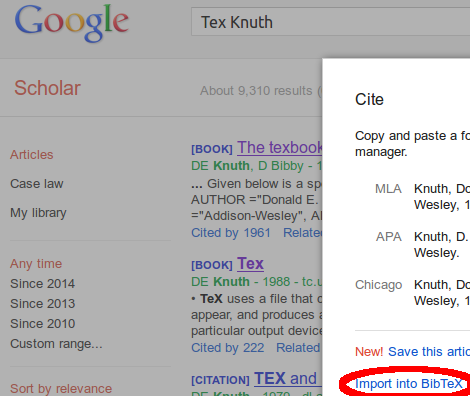
\includegraphics[width=\textwidth]{img/scholar_circle.png}
\end{column}
\end{columns}

\begin{description}
  \item[bad] \lstinline|voir\cite{goossens93}|
  \item[ok] \lstinline|voir \cite{goossens93}|
  \item[ok] \lstinline|voir~\cite{goossens93}|
\end{description}

\bibliographystyle{plain}
  \begin{block}{Élément d'une bibliographie}
    À mettre dans \lstinline|biblio.bib|
    \begin{lstlisting}
@book{goossens93,
    author    = "Michel Goossens and Frank Mittelbach and Alexander Samarin",
    title     = "The LaTeX Companion",
    year      = "1993",
    publisher = "Addison-Wesley",
    address   = "Reading, Massachusetts"
}
@book{knuth1986texbook,
  title={The texbook},
  author={Knuth, Donald Ervin and Bibby, Duane},
  volume={1993},
  year={1986},
  publisher={Addison-Wesley Reading, MA, USA}
}
    \end{lstlisting}
  \end{block}
\end{frame}


\subsection{Découpe d'un projet en fichiers}
\begin{frame}[fragile]
  \frametitle{Découpe d'un projet en fichiers}
  \begin{itemize}
    \item Si vous travaillez sur un projet de moyenne ou grande envergure, il vaut la peine de le découper en plusieurs fichiers
    \item Cela accélère la recompilation et permet une séparation plus claire entre les sections
    \item Par exemple, un roman pourrait avoir un fichier par chapitre:
    \begin{itemize}
      \item \texttt{roman.tex} contient la structure du projet;
      \item \texttt{entete.tex} contient l'en-tête \LaTeX{};
      \item \texttt{intro.tex} contient l'introduction et les remerciements;
      \item \texttt{chap1.tex} contient le premier chapitre et son titre;
      \item \texttt{chap2.tex} contient le deuxième chapitre et son titre;
      \item \dots
    \end{itemize}
  \end{itemize}
\end{frame}

\subsection{Découpe d'un projet en fichiers}
\begin{frame}[fragile]
  \frametitle{Découpe d'un projet en fichiers}
  \framesubtitle{input et include}
  \begin{itemize}
    \item Deux commandes permettent l'inclusion d'un fichier dans un autre: \lstinline|\input{}| et \lstinline|\include{}|
    \item On leur donne en argument le nom du fichier sans le \texttt{.tex}
    \item \lstinline|\input{}| \og{}copie\fg{} le document littéralement
    \item \lstinline|\include{}| termine la page courante, copie le document, puis termine la page courante à nouveau
    \item \lstinline|\input{}| peut se trouver n'importe où, y compris dans le préambule, tandis que \lstinline|\include{}| doit se trouver dans le corps du document
    \item \lstinline|\include{}| accélère la compilation du document, car cela permet de ne recompiler que ce qui a été modifié
    \item La commande \lstinline|\includeonly{doc1,doc2,...}| permet de restreindre les documents à inclure
  \end{itemize}
\end{frame}

\subsection{Découpe d'un projet en fichiers}
\begin{frame}[fragile]
  \frametitle{Découpe d'un projet en fichiers}
  \framesubtitle{Exemple du roman}
  \begin{columns}
    \begin{column}{0.5\textwidth}
      Dans \texttt{roman.tex}
      \begin{lstlisting}[style=nonumbers]
\documentclass[a4paper]{book}

\input{entete}

\begin{document}
  \maketitle
  \tableofcontents
  
  \includeonly{intro,chap2} % Inclure uniquement ces fichiers-ci
  
  \include{intro}
  \include{chap1}
  \include{chap2}
  ...
\end{document}
      \end{lstlisting}
    \end{column}
    \begin{column}{0.5\textwidth}
      Dans \texttt{entete.tex}
      \begin{lstlisting}[style=nonumbers]
\usepackage[utf8x]{inputenc}
\usepackage[T1]{fontenc}
\usepackage[french]{babel}
...
      \end{lstlisting}
      
      Dans \texttt{intro.tex}
      \begin{lstlisting}[style=nonumbers]
\begin{center}
  Je dédie ce roman à mon chat.
  Tu nous a quitté trop vite, Dragibus.
  Repose en paix.
\end{center}
      \end{lstlisting}
      
      Dans \texttt{chap1.tex}
      \begin{lstlisting}[style=nonumbers]
\chapter{Le début d'une histoire
         trépidante!...}
...
      \end{lstlisting}
    \end{column}
  \end{columns}
\end{frame}


%-----------------------
\section{Sciences}
\subsection{Écrire des mathématiques}
\begin{frame}[fragile]{L'environnement mathématique}
\framesubtitle{Inclure des formules dans le texte}
\begin{itemize}
	\item On peut ajouter une formule mathématique dans du texte entre deux symboles \textbf{\$} ou entre \lstinline|\( ... \)|.

\begin{center}
  \begin{tabular}{lll}
    \lstinline|$x + 1 = 2$| & $x + 1 = 2$\\
    \medskip
    \lstinline|$\frac{1}{x}$| & $\frac{1}{x}$\\
  \end{tabular}
\end{center}
	\item Les opérateurs, symboles,\dots commencent par \textbf{\textbackslash}, sauf \lstinline|+, -, /, ^, _,...|.
	\begin{center}
		\begin{tabular}{llr}
			\lstinline|$a^{11}$| & $a^{11}$ & Good \\
			\lstinline|$a^11$| & $a^11$ & Bad ! \\
			\lstinline|$\sin(x)$| & $\sin(x)$ & Good \\
			\lstinline|$sin(x)$| & $sin(x)$ & Bad !\\
			\lstinline|$\frac{\Theta}{\sqrt{\beta}}$| & $\frac{\Theta}{\sqrt{\beta}}$ & 
		
		\end{tabular}
	\end{center}
	\item Les packages \lstinline|amsmath| et \lstinline|amssymb| apportent beaucoup d'envirronement et symboles supplémentaires très utiles, à inclure par défaut.
\end{itemize}
\end{frame}

\begin{frame}[fragile]{L'environnement mathématique}
\framesubtitle{Inclure des formules centrées hors du texte}

\begin{itemize}
\item On peut aussi ajouter une formule mathématique centrées hors du texte entre deux symboles \textbf{\$\$} ou entre \lstinline|\[ ... \]|.
\vspace{0.5cm}
\begin{columns}
  \begin{column}{0.45\textwidth}
    L'expression $\sin(x)$ peut s'écrire de différents manières. En effet, il a été démontré que 
    
    $$\sin(x) = \frac{e^{iz} - e^{-iz}}{2i}$$

    avec $i$ étant l'unité imaginaire.
  \end{column}
  \begin{column}{0.45\textwidth}
    \begin{lstlisting}[style = nonumbers]
L'expression $\sin(x)$ peut s'écrire de différents manières. En effet, il a été démontré que 

$$\sin(x) = \frac{e^{iz} - e^{-iz}}{2i}$$

avec $i$ étant l'unité imaginaire.
    \end{lstlisting}
  \end{column}
\end{columns}

\end{itemize}
\end{frame}
\subsection{Matrices}
\begin{frame}[fragile]{Matrices}
	\begin{itemize}
		\item Les matrices s'écrivent avec l'environnement \lstinline|matrix| (fonctionnement semblable à \lstinline|tabular|).
			\begin{columns}
				\begin{column}{0.45\textwidth}
					$$\begin{matrix}
						\alpha & \beta \\
						\gamma & \delta \\
					\end{matrix}$$
				\end{column}
				\begin{column}{0.45\textwidth}
					\begin{lstlisting}[style=nonumbers]
$$\begin{matrix}
\alpha & \beta \\
\gamma & \delta \\
\end{matrix}$$
					\end{lstlisting}
				\end{column}
			\end{columns}
		\item Les commandes \lstinline|\left| et \lstinline|\right| permettent de changer les délimiteurs de la matrice.
			\begin{columns}
				\begin{column}{0.45\textwidth}
					$$\left\{
					\begin{array}{r c l}
						a + b & = & c \\
						d & = & e + f \\
					\end{array}
					\right.$$
				\end{column}
				\begin{column}{0.45\textwidth}
					\begin{lstlisting}[style=nonumbers]
$$\left\{
\begin{array}{r c l}
a + b & = & c \\
d & = & e + f \\
\end{array}
\right.$$
					\end{lstlisting}
				\end{column}
			\end{columns}
	\end{itemize}
\end{frame}

\subsection{Formles numérotées}
\begin{frame}[fragile,allowframebreaks]{Formules numérotées}

\begin{itemize}
	\item L'environnement \lstinline|align| permet d'écrire des équations alignées et numérotées.
	\item On peut ne pas numéroter une équation en plaçant \lstinline|\nonumber| à la fin de la ligne. 
	
	\vspace{0.50cm}
\begin{columns}
  \begin{column}{0.45\textwidth}
I like trains and the equations
\begin{align}
  e^{i\pi} + 1 & = 0\\
  f(t) & = A\cos(\omega t + \phi) \nonumber 
\end{align}
I also know that
\begin{align*}
  1 + 1 & = 2\\
  2 + 3 & = 5
\end{align*}
  \end{column}
  \begin{column}{0.4\textwidth}
    \begin{lstlisting}[style = nonumbers]
I like trains and the equations
\begin{align}
  e^{i\pi} + 1 & = 0\\
  f(t) & = A\cos(\omega t + \phi) \nonumber 
\end{align}
I also know that
\begin{align*}
  1 + 1 & = 2\\
  2 + 3 & = 5
\end{align*}
    \end{lstlisting}
  \end{column}
\end{columns}
\framebreak
\item Possibilité de référencer les équation en plaçant \lstinline|\label| à la fin de la ligne dans l'environnement \lstinline|align|.
\vspace{0.5cm}
	\begin{columns}
		\begin{column}{0.5\textwidth}
			We see in equation~\ref{first} that $x$ is smaller than $3$ and in equation~\ref{third} that $y$ is greater than $x$. 
			\begin{align}
				x & < 3 \label{first} \\
				y & > 5 \label{second} \\
				y & > x \label{third}
			\end{align}
		\end{column}
		\begin{column}{0.5\textwidth}
		\begin{lstlisting}[style=nonumbers]
We see in equation~\ref{first} that $x$ is smaller than $3$ and in equation~\ref{third} that $y$ is greater than $x$. 
\begin{align}
x & < 3 \label{first} \\
y & > 5 \label{second} \\
y & > x \label{third}
\end{align}
		\end{lstlisting}
		\end{column}
	\end{columns}
\end{itemize}
\end{frame}

\subsection{Les maths et les polices}
\begin{frame}[fragile]{Les maths et les polices}
\begin{itemize}
	\item Parfois, certaines variables sont composées de plusieurs lettres. On doit utiliser des polices différentes comme \lstinline|\mathrm| ou \lstinline|\mathsf|. \lstinline|\mathcal| produit des lettres \og calligraphiques \fg{}. 
	\begin{center}
			\begin{tabular}{lll}
				\lstinline|$Var(x)$| & $Var(x)$ & Bad ! \\
				\lstinline|$\mathrm{Var}(x)$| & $\mathrm{Var}(x)$ & Good \\
				\lstinline|$\mathcal{M}$| & $\mathcal{M}$ &
			\end{tabular}
	\end{center}
	
	\item Pour les intégrales, le \og dx \fg{} ne s'écrit pas n'importe comment.
	\begin{center}
			\begin{tabular}{ll}
				\lstinline|$\int y \,\mathrm{d}x$| & $\int y \,\mathrm{d}x$\\
			\end{tabular}
	\end{center}
	\item Les ensembles s'écrivent à l'aide de la police \lstinline|\mathbb|.
	\begin{center}
		\begin{tabular}{cccc}
		\lstinline|$\mathbb{N}$| & $\mathbb{N}$ & \lstinline|$\mathbb{Z}$| & $\mathbb{Z}$ \\
		\lstinline|$\mathbb{D}$| & $\mathbb{D}$ & \lstinline|$\mathbb{Q}$| & $\mathbb{Q}$ \\
		\lstinline|$\mathbb{N}$| & $\mathbb{R}$ & \lstinline|$\mathbb{C}$| & $\mathbb{C}$			
		\end{tabular}
	\end{center}
\end{itemize}	
\end{frame}

\subsection{Large Operators}
\begin{frame}[fragile,allowframebreaks]{Large Operators}
\begin{itemize}
	\item Ces opérateurs mathématiques sont $\lim, \min, \max, \sum, \prod, \ldots$.
	
Quelle différence ? Leurs indices et exposant sont au dessus et en dessous et pas à leur droite.
	\item Dans un texte, on obtient 
	$\min_{x \in \mathbb{R}^n} \|x\| \text{~tel que~} \sum_{i = 1}^n x_i = 1$
\begin{lstlisting}[style=nonumbers]
Dans un texte, on obtient 
$\min_{x \in \mathbb{R}^n} \|x\| \text{tel que} \sum_{i = 1}^n x_i = 1$
\end{lstlisting}

	\item Dans une équation, le résultat est : $$\min_{x \in \mathbb{R}^n} \|x\| \text{tel que} \sum_{i = 1}^n x_i = 1$$
\begin{lstlisting}[style=nonumbers]
Dans une équation, le résultat est : 
$$\min_{x \in \mathbb{R}^n} \|x\| \text{tel que} \sum_{i = 1}^n x_i = 1$$
\end{lstlisting}
\framebreak
	\item Pour quand même placer les indices/exposants au dessus/dessous, utiliser \lstinline|\limits| juste après l'opérateur.
	\begin{center}
	\begin{tabular}{ll}
	\lstinline|$\min\limits_{x \in \mathbb{R}^n} x$| & $\min\limits_{x \in \mathbb{R}^n} x$\\
	& \\
	\lstinline|$\sum\limits_{i = 1}^n x_i = 1$| & $\sum\limits_{i = 1}^n x_i = 1$
	\end{tabular}
	\end{center}
\end{itemize}
\end{frame}

%TODO : Exemple plus simple et \operatorname{}
\begin{frame}[fragile]{L'environnement mathématique}
\framesubtitle{Définition de commandes, plus d'excuse !}
\label{noexcuse}
\begin{lstlisting}
\newcommand{\fin}{\mathsf{flux}_{\text{in}}}
\newcommand{\fout}{\mathsf{flux}_{\text{out}}}
% if \kor already exists
\renewcommand{\kor}{k_{\text{orig}}}
\newcommand{\kde}{k_{\text{dest}}}
\DeclareMathOperator{\pot}{potato} % mieux que \newcommand{\mathop{\mathrm{..}}}
% \min already exists: Trick for ``reDeclareMathOperator''
\let\min\relax% Set equal to \relax so that LaTeX thinks it's not defined
\DeclareMathOperator{\min}{minimum}
\newcommand{\badet}{et}
\newcommand{\goodet}{\mathbin{\mathrm{et}}}
\end{lstlisting}
\begin{columns}
  \begin{column}{0.45\textwidth}
    \begin{lstlisting}
\[ \alpha >> \beta \badet <x,y> = 0 => \]
    \end{lstlisting}
  \end{column}
  \begin{column}{0.35\textwidth}
    \[ \alpha >> \beta \badet <x,y> = 0 => \]
  \end{column}
  \begin{column}{0.2\textwidth}
    
\includegraphics[height=3em]{i_dont_want_to_live_on_this_planet_anymore.jpg}
  \end{column}
\end{columns}
\begin{columns}
  \begin{column}{0.45\textwidth}
    \begin{lstlisting}
\[ \alpha \gg \beta \goodet \langle x,y \rangle = 0 \Rightarrow \]
    \end{lstlisting}
  \end{column}
  \begin{column}{0.35\textwidth}
    \[ \alpha \gg \beta \goodet \langle x,y \rangle = 0 \Rightarrow \]
  \end{column}
  \begin{column}{0.2\textwidth}
    
\includegraphics[height=3em]{success_kid.jpg}
  \end{column}
\end{columns}
\end{frame}

\begin{frame}[fragile]{L'environnement mathématique}
\framesubtitle{Forcer un espacement}
Rarement utile !

\begin{center}
  \begin{tabular}{ll}
    Commande & espacements en mu (espace normal${}={}$6mu)\\
    \hline
    \lstinline|\!|     & $-$3\\
    \lstinline|\,|     &  3\\
    \lstinline|\:|     &  4\\
    \lstinline|\;|     &  5\\
    \lstinline|\ |     &  6\\
    \lstinline|\quad|  & 18\\
    \lstinline|\qquad| & 36
  \end{tabular}
\end{center}
\end{frame}

\begin{frame}[fragile]{L'environnement mathématique}
\framesubtitle{Forcer un espacement : Exemples}
\begin{columns}
  \begin{column}{0.5\textwidth}
    \begin{lstlisting}
\begin{align*}
  a & = u + v + w + x + y\\
    & \quad + z
\end{align*}
    \end{lstlisting}
  \end{column}
  \begin{column}{0.5\textwidth}
\begin{align*}
  a & = u + v + w + x + y\\
    & \quad + z
\end{align*}
  \end{column}
\end{columns}

Erreur courante: les ensembles besoin d'espacement (i.e. \lstinline|\,|) en compréhension mais pas en extension.
\begin{columns}
  \begin{column}{0.5\textwidth}
    \begin{lstlisting}
\begin{align*}
  \mathbb{R}_+ & = \{\, x \in \mathbb{R} \mid R \geq 0 \,\}\\
  \mathbb{R}_+ & = \{\, x \in \mathbb{R} : R \geq 0 \,\}\\
  \mathbb{N} & = \{0, 1, 2, 3, 4, \ldots\}\\
\end{align*}
    \end{lstlisting}
  \end{column}
  \begin{column}{0.5\textwidth}
\begin{align*}
  \mathbb{R}_+ & = \{\, x \in \mathbb{R} \mid R \geq 0 \,\}\\
  \mathbb{R}_+ & = \{\, x \in \mathbb{R} : R \geq 0 \,\}\\
  \mathbb{N} & = \{0, 1, 2, 3, 4, \ldots\}\\
\end{align*}
  \end{column}
\end{columns}
\end{frame}

\subsection{La physique}
\begin{frame}[fragile]
  \frametitle{Les unités}
  \lstinline|\usepackage{siunitx}|
  \begin{center}
    \begin{tabular}{ll}
      \num{314e-2} & \lstinline|\num{314e-2}|\\
      \ang{42} & \lstinline|\ang{42}|\\
      \si{g_{polymer}~mol_{cat}.s^{-1}} &
      \lstinline|\si{g_{polymer}~mol_{cat}.s^{-1}}|\\
      \si{\square\volt\cubic\lumen\per\farad} &
      \lstinline|\si{\square\volt\cubic\lumen\per\farad}|\\
      \SI{e-6}{\meter\per\second\per\ohm} &
      \lstinline|\SI{e-6}{\meter\per\second\per\ohm}|\\
      \SI[per-mode=symbol]{5.3e9}{m\per s} &
      \lstinline|\SI[per-mode=symbol]{5.3e9}{m\per s}|\\
      \SI[per-mode=symbol]{5.3e9}{\meter\per\second\per\ohm} &
      \lstinline|\SI[per-mode=symbol]{5.3e9}{\meter\per\second\per\ohm}|\\
      \SI[per-mode=fraction]{5e6}{\joule\per\second} &
      \lstinline|\SI[per-mode=fraction]{5e6}{\joule\per\second}|\\
      \SI{-273.15}{\celsius} &
      \lstinline|\SI{-273.15}{\celsius}|
    \end{tabular}
  \end{center}
  Super doc sur \url{http://ctan.org/pkg/siunitx}
\end{frame}

\subsection{La chimie}
\begin{frame}[fragile]
  \centering
  \frametitle{La chimie}
  \begin{lstlisting}
\usepackage{chemfig}
...
\chemfig{*6(-=(-CH_2OH)-(-COOH)=-=)}
  \end{lstlisting}
  \begin{center}
    \chemfig{*6(-=(-CH_2OH)-(-COOH)=-=)}
  \end{center}
  \begin{lstlisting}
\usepackage[version=3]{mhchem}
...
$$\ce{3H2O + 1/2H2O -> AgCl2- + H2_{(aq)}}$$
  \end{lstlisting}
  $$\ce{3H2O + 1/2H2O -> AgCl2- + H2_{(aq)}}$$
\end{frame}

\subsection{Les circuits}
\begin{frame}[fragile]
  \frametitle{Les circuits}
  \begin{lstlisting}
    \usepackage{circuitikz}
    ...
		\shorthandoff{:!} % Pour certaines versions de circuitikz
    \begin{circuitikz}
      \draw (0,0) to [sI, v=$V_2$] (0,-3);
      \draw (6,-3) to[short, i = $I_2$] (0,-3);
      \draw (0,0) to [R = R, v = $V_R$] (3,0);
      \draw (3,0) to [L = L, v = $V_L$] (6,0);
      \draw (6,0) to [C = C, v = $V_C$] (6,-3);
    \end{circuitikz}
		\shorthandon{:!} % Pour certaines versions de circuitikz
  \end{lstlisting}
  \begin{center}
		\shorthandoff{:!}
    \begin{circuitikz}
      \draw (0,0) to [sI, v=$V_2$] (0,-3);
      \draw (6,-3) to[short, i = $I_2$] (0,-3);
      \draw (0,0) to [R = R, v = $V_R$] (3,0);
      \draw (3,0) to [L = L, v = $V_L$] (6,0);
      \draw (6,0) to [C = C, v = $V_C$] (6,-3);
    \end{circuitikz}
		\shorthandon{:!}
  \end{center}
\end{frame}

\subsection{Inclure du code}
\begin{frame}[fragile]
  \frametitle{Inclure du code}
  \begin{lstlisting}[mathescape=true]
\begin{lstlisting}
if a == b:
  return 0
else:
  return 1
\$$end{lstlisting}
  \end{lstlisting}
donne
  \begin{lstlisting}[language=Python]
if a == b:
  return 0
else:
  return 1
  \end{lstlisting}

  Il y a aussi
  \begin{lstlisting}
\lstinputlisting[caption={...},label=...]{main.py}
  \end{lstlisting}
  et
  \begin{lstlisting}
\lstinline|if a == b|
  \end{lstlisting}
  qui donne \lstinline[language=Python]|if a == b|.
\end{frame}

%%%%%%%%%%%%%

\AtBeginSection[]{} %% stop TOC

\section{Exercices}
\begin{frame}
\frametitle{Exerçons-nous}
	\begin{itemize}
		\item<1-> Télécharger le document \textbf{exemple.pdf}
		\item<2-> Reproduire une structure similaire :
			\begin{itemize}
				\item page de titre
				\item table des matières
				\item liste, tableau, figure
				\item math en ligne, hors-ligne
				\item références
				\item \dots
			\end{itemize}
		\item<3-> Chercher de l'information :
			\begin{itemize}
				\item \url{http://en.wikibooks.org/wiki/LaTeX}
				\item \url{http://www.grappa.univ-lille3.fr/FAQ-LaTeX}
                \item \url{http://www.andy-roberts.net/writing/latex}
                \item \url{http://ctan.org/pkg/packagename} ou \lstinline[language=sh,morekeywords={texdoc}]{$ texdoc packagename}
				\item Google est ton ami !
                \item \url{http://www.sharelatex.com/learn}
                \item La version de StackExchange spécialisée pour le \TeX:
      \url{tex.stackexchange.com}.
				\item Livres:
				\begin{itemize}
					\item \LaTeX HowTo par Sébastien Combéfis (EN/FR)
					\item Framabook \LaTeX
				\end{itemize}
				\item \url{http://www.tablesgenerator.com/}
			\end{itemize}
	\end{itemize}
\end{frame}


\end{document}
